%%%%%%%% ICML 2026 SHARED WORKSHOP DRAFT %%%%%%%%%%%%%%%%%

\documentclass{article}

\usepackage{microtype}
\usepackage{graphicx}
\usepackage{subcaption}
\usepackage{booktabs}
\usepackage{array}
\usepackage{hyperref}
\newcommand{\theHalgorithm}{\arabic{algorithm}}
\usepackage{icml2026}
\usepackage{amsmath}
\usepackage{amssymb}
\usepackage{mathtools}
\usepackage{amsthm}
\usepackage[capitalize,noabbrev]{cleveref}
\usepackage{placeins}

\newcommand{\dataset}{\mathcal{D}}
\newcommand{\conditions}{\mathcal{C}}
\newcommand{\package}{\mathcal{E}}
\newcommand{\auditor}{\mathcal{A}_{\theta}}

\icmltitlerunning{White Box Evidence Packages for Policy Audit Reports}

\begin{document}

\twocolumn[
  \icmltitle{White Box Evidence Packages for Policy Audit Reports}

  \begin{icmlauthorlist}
    \icmlauthor{Anonymous Authors}{anon}
  \end{icmlauthorlist}
  \icmlaffiliation{anon}{Anonymous Institution}
  \icmlcorrespondingauthor{Anonymous Authors}{anonymous@example.com}
  \icmlkeywords{mechanistic interpretability, AI auditing, technical AI governance, sparse autoencoders, white box evaluation}

  \vskip 0.3in
]

\printAffiliationsAndNotice{}

\begin{abstract}
Policy audits of language models often rely on surface text and output summaries, but governance practice increasingly asks for traceability, verification, and documented evidence. We study whether white box evidence packages change reports produced by an independent auditor model. The experiment is deliberately not a retrieval benchmark: the unit of evaluation is the audit report and its evidence use. We construct 60 policy audit cases from AGORA and generate 600 structured reports with a local Qwen 2.5 7B auditor across ten evidence conditions. We then conduct pilot human review on 20 paired cases for black box surface evidence, full white box evidence, hybrid evidence, and a shuffled white box control. Full white box evidence increases cited evidence ids relative to black box evidence, with 10.13 versus 3.87 cited ids per report, but human review shows lower average correctness (3.85 vs. 4.30), weaker span grounding (2.85 vs. 3.75), and higher evidence misuse (2.55 vs. 1.00). Hybrid evidence performs best on average correctness and usefulness (4.55 and 4.60), while still increasing misuse relative to black box evidence (1.55 vs. 1.00). The shuffled control is the main governance warning: it scores 4.35 on evidence misuse, and 11 of 20 shuffled reports have both high correctness and high misuse. White box evidence can make audit reports more traceable, but only when the interface anchors internal evidence to passage evidence and tests relevance with controls.
\end{abstract}

\section{Introduction}

AI governance increasingly relies on audits that can be inspected by actors outside the model developer. Policy regimes ask for assessment, access, verification, monitoring, and accountability, but many technical methods still produce benchmark scores or output summaries rather than auditable evidence trails \citep{reuel2024technical,reuelbucknall2024open,ojewale2025accountability}. Black box access remains essential because it reflects what external users can observe, but it is not always enough for policy oversight. The question is not simply whether an auditor can ask a model more questions. It is whether the audit record makes clear what evidence was available, what evidence was used, and where the evidence could be wrong.

This paper therefore studies a narrow audit interface question. Given the same policy passage and audit rubric, how do black box evidence and white box evidence packages change the report produced by an independent auditor LLM? We do not frame the task as retrieval. A retrieval system may find related policy families while still failing to produce a traceable audit artifact. Our unit of analysis is the report: its findings, cited evidence ids, passage spans, confidence, and misuse of evidence. The central claim is deliberately conservative. White box evidence changes auditor evidence use and can make reports more traceable, but uptake is not validity. In our pilot, full white box evidence alone worsens grounded audit quality relative to a strong black box surface baseline, while a hybrid interface is more promising because it keeps passage evidence in control and treats internal evidence as secondary.

\Cref{fig:package-design} summarizes the design. We construct 60 AGORA policy cases, generate 600 structured reports with a local auditor across ten evidence conditions, and conduct human gold review on 20 paired cases for the primary interfaces. This gives three linked contributions. First, we define a policy audit report experiment that compares evidence interfaces rather than retrieval systems. Second, we instantiate a multi tool white box package using SAE features, logit lens outputs, steering evidence, and activation explanation surrogates. Third, we show why negative controls matter: shuffled white box evidence can produce plausible reports with invalid internal citations. To support anonymous review and reproducibility, we provide an anonymized artifact repository with code, prompts, evidence packages, final reports, human review files, and paper figures at \url{https://anonymous.4open.science/r/agora-mi-C473/README.md}.

\begin{figure*}[t]
    \centering
    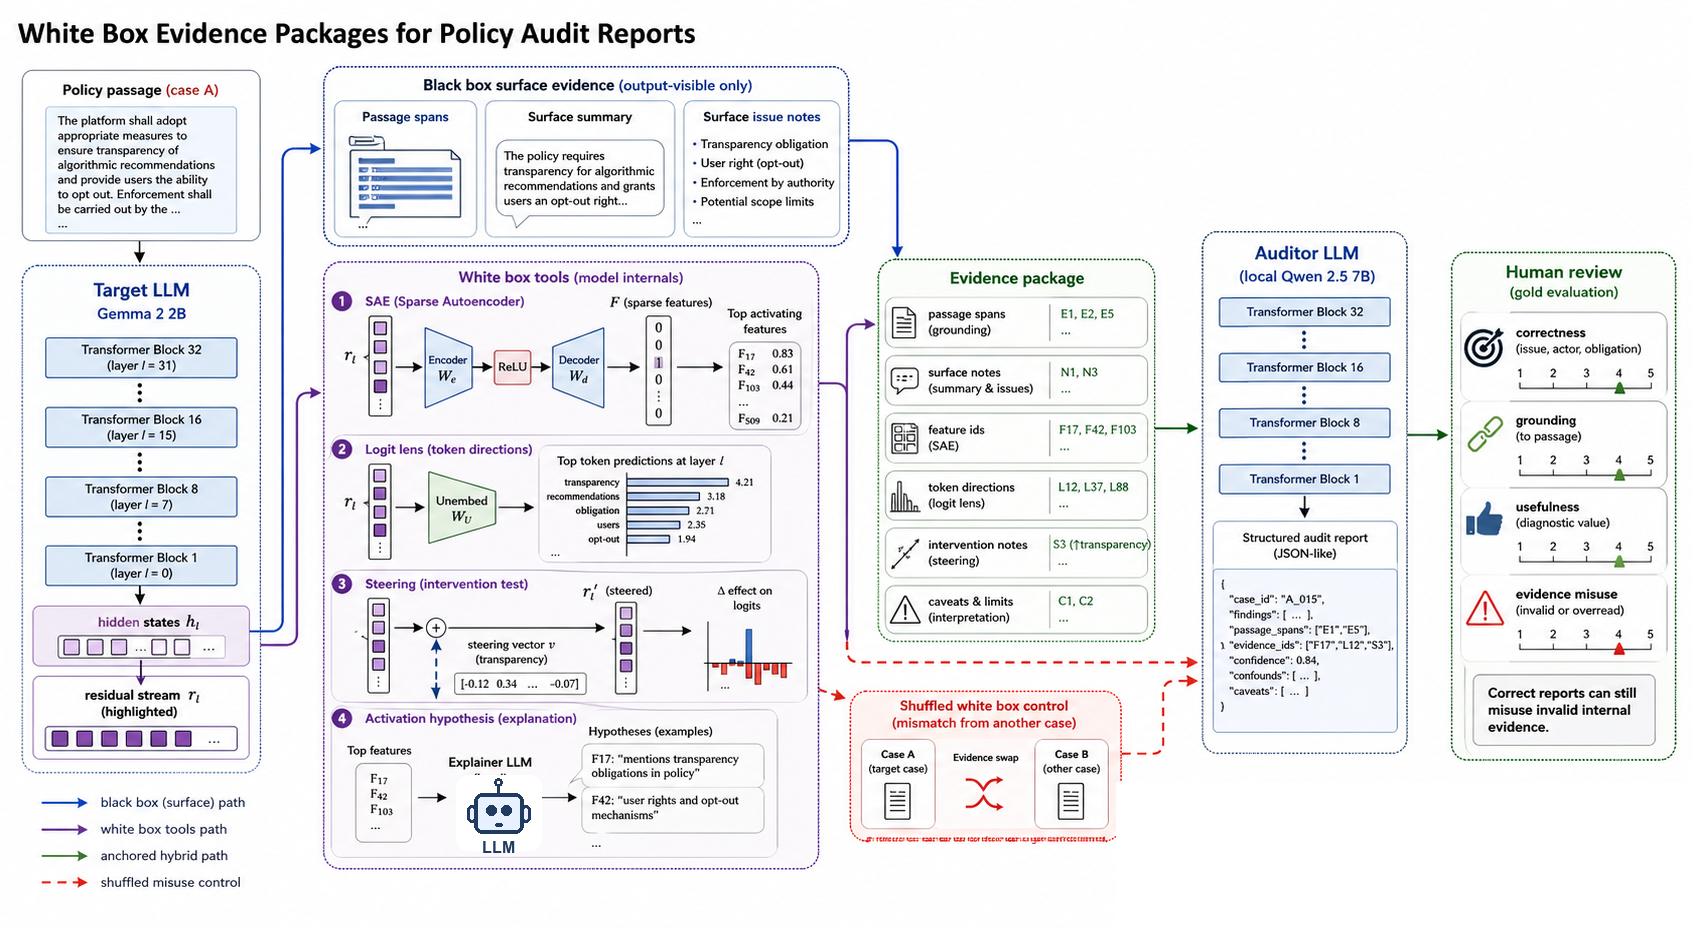
\includegraphics[width=0.98\textwidth]{figures/audit_evidence_package_design_transformer.png}
    \caption{Evidence package audit design. Policy passages are processed by a target model, internal states are summarized through SAE, logit lens, steering, and activation hypothesis tools, and the resulting evidence package is given to an auditor model. The unit of comparison is the evidence interface, not a retrieval system. Human gold briefs are written from the policy passage before diagnostic review of auditor reports.}
    \label{fig:package-design}
\end{figure*}

\section{Related Work}

Technical AI governance work argues that oversight institutions need tools for access, assessment, verification, and accountability rather than only post hoc descriptions of model outputs \citep{reuel2024technical,reuelbucknall2024open,ojewale2025accountability}. Related audit access work argues that black box interaction can miss information needed to test developer claims and system risks, motivating controlled access to weights, activations, development evidence, or verification channels \citep{casper2024blackbox,waiwitlikhit2024trustless,harack2025verification}. Our study takes that access argument seriously but evaluates access as an evidence interface: internal information must be packaged, cited, and tested before it can support an audit report.

Audit practice also motivates the interface view. Assurance standards and regulatory audit regimes ask auditors to connect conclusions to sufficient and appropriate evidence, while early DSA audit critiques highlight that formal audit reports can remain weak when audit criteria, evidence relevance, and systemic risk tests are underspecified \citep{iaasb2013isae3000,solarova2026checkbox,holznagel2025dsa}. Access scholarship similarly warns that API and platform restrictions can create audit blind spots even when transparency mandates exist \citep{burnat2025accountability,cen2024transparency}. Stakeholder first transparency work argues that explanations should be tailored to the decision maker and use context rather than treated as generic disclosures \citep{bell2022stakeholders}. We apply these ideas to auditor facing LLM reports: the evidence package must support traceability, relevance checking, and review of how evidence was used.

Mechanistic interpretability offers candidate tools for that interface, but the tools do not become valid audit evidence merely because they expose internals. Sparse autoencoders can turn residual stream activations into feature hypotheses \citep{cunningham2024sae,bricken2023monosemanticity,templeton2024scaling,lieberum2024gemmascope}; logit lens methods can summarize intermediate token directions \citep{belrose2023tunedlens}; steering and sensitivity methods can test how internal directions affect model behavior \citep{cyberey2026steering}; and automated explanation methods can convert activations into natural language hypotheses \citep{bills2023neurons,activationoracles2025}. Recent evaluation work warns that readable labels and tool outputs should be tested through downstream use, ablations, and controls rather than treated as explanations by default \citep{karvonen2025saebench,sheshadri2026auditbench}. AuditBench is closest in spirit because it evaluates multiple white box tools as audit instruments; our setting differs by moving the unit of evaluation from tool success on model behavior audits to the downstream policy report artifact, where the same passage and rubric are held fixed and the evidence interface is varied. This warning is especially important in policy text, where a report can sound correct by leaning on generic legal language while missing the actual actor, obligation, exception, or remedy.

\section{Audit Task and Evidence Interfaces}

Each case consists of a policy passage, a fixed audit rubric, and a hidden gold brief. The auditor is asked to identify policy relevant issues, cite supplied evidence ids and exact passage spans, record uncertainty, and avoid claims not supported by the package. The report is not a legal compliance decision. It is an evidence artifact for later review. This distinction matters because policy passages contain many plausible but confounded cues. A report can correctly recognize that a provision concerns transparency or risk management while still misidentifying who has the obligation, whether the text creates a right or an exception, or whether a cited internal signal is actually relevant.

Formally, let $\dataset=\{(x_i,m_i,g_i)\}_{i=1}^{N}$ be policy passages $x_i$, metadata $m_i$, and hidden gold briefs $g_i$. For each evidence condition $c\in\conditions$, the package builder emits
\begin{align}
\package_{i,c} &= \{e_{i,c,1},\ldots,e_{i,c,M_{i,c}}\},\\
y_{i,c} &= \auditor(x_i,r,\package_{i,c}),
\end{align}
where $r$ is the fixed audit rubric and $y_{i,c}$ is a structured report. The report contains findings $\hat{G}_{i,c}$, cited passage spans $S_{i,c}$, cited evidence ids $Z_{i,c}\subseteq\{id(e):e\in\package_{i,c}\}$, confidence $q_{i,c}$, and uncertainty notes $u_{i,c}$. The experiment therefore asks how changing $\package_{i,c}$ changes $y_{i,c}$ while holding $x_i$, $r$, and $\auditor$ fixed.

The package builder creates one auditor facing record for each condition case pair. Every record contains the passage, the same rubric, a condition neutral instruction, and condition specific evidence items with stable ids, evidence types, source fields, text fields, and caveats. The auditor is asked to cite ids only when they directly support a finding. This design separates three objects that are often conflated: passage evidence, surface or black box observations, and internal evidence about the target model.

C1 is intentionally strong rather than empty, but it remains a text only black box interface. It is built by splitting the policy passage into sentences $s$ and scoring each sentence with an audit cue lexicon $T$:
\begin{equation}
b(s)=\sum_{\tau\in T}\mathbf{1}[\tau \text{ occurs in } s].
\end{equation}
The top scoring sentences become surface evidence items with selected spans, issue notes, confidence fields, and explicit caveats that no hidden state was used. This makes C1 a surface evidence scaffold rather than an internal access condition.

\Cref{tab:conditions} lists the ten evidence conditions. C6 combines all available white box views. C7 tests the practical interface where surface anchors and internal evidence are supplied together. C9 preserves the shape of the full white box package while drawing evidence from another case. It is not a normal baseline; it is the control that tells us whether the auditor treats plausible looking internal evidence as authoritative when relevance is broken.

\begin{table}[h!]
    \centering
    \caption{Evidence conditions.}
    \label{tab:conditions}
    \scriptsize
    \setlength{\tabcolsep}{3pt}
    \begin{tabular}{@{}p{0.11\columnwidth}p{0.25\columnwidth}p{0.56\columnwidth}@{}}
        \toprule
        ID & Interface & Auditor facing contents \\
        \midrule
        C0 & Passage & Passage and rubric only. \\
        C1 & Black box & Surface summary, selected spans, issue notes, and confidence. \\
        C2 & SAE & Feature ids, layers, activations, labels, spans, and caveats. \\
        C3 & Logit lens & Intermediate token direction summaries. \\
        C4 & Steering & Directional sensitivity and output or score deltas. \\
        C5 & Surrogate & Natural language activation hypotheses. \\
        C6 & Full white box & C2 through C5 together. \\
        C7 & Hybrid & C1 plus C6. \\
        C8 & Raw SAE & Raw AutoInterp labels and feature ids. \\
        C9 & Shuffled & C6 style evidence drawn from another case. \\
        \bottomrule
    \end{tabular}
\end{table}

The white box package is multi tool because each tool answers a different evidence question. SAE features identify sparse concept like activations and where they peak in the passage. Logit lens records describe intermediate token directions. Steering records describe sensitivity under a selected contrast direction. The activation explanation surrogate converts selected activation evidence into a natural language hypothesis, but we label it as a surrogate rather than a validated Activation Oracle. The paper treats all of these as evidence items for review, not as final conclusions about model reasoning.

For target residual state $h_{i,l,p}$ at layer $l$ and token position $p$, SAE evidence uses feature activations $a_{i,l,k,p}$ and reports the maximum activation $A_{i,l,k}=\max_p a_{i,l,k,p}$ with its peak token span. Logit lens evidence maps the same hidden state into vocabulary space, $\ell_{i,l,p}=W_U\mathrm{LN}(h_{i,l,p})$, and reports top token directions rather than final model outputs. Steering evidence uses a contrast direction $v_l=(\mu_l^{+}-\mu_l^{-})/\|\mu_l^{+}-\mu_l^{-}\|_2$ and probes $h'_{i,l,p}=h_{i,l,p}+\alpha\|h_{i,l,p}\|_2v_l$ with $\alpha=0.35$. These definitions are intentionally lightweight: they specify what the auditor sees, while the human review tests whether the resulting citations are valid for the policy report.

\FloatBarrier

\section{Experimental Setup}

We use 60 policy cases drawn from AGORA, a corpus of AI governance and regulatory material \citep{arnold2024agora}. The cases cover six policy families with ten cases per family. The interpreted target model is Gemma 2 2B, and the auditor is a local Qwen 2.5 7B model run with structured JSON output. For each condition, the auditor receives only the passage, rubric, and assigned evidence package. It does not see the hidden gold brief and is not told that C9 contains shuffled evidence.

The package generator is deterministic given the selected case set. SAE items use Gemma Scope residual stream SAEs and human revised AutoInterp labels where available. Logit lens items use Gemma 2 2B layers 6, 12, 18, and 24 at audit cue token positions selected from the passage. Steering items use layers 12, 18, and 24 with a fixed obligation and risk contrast prompt set. The activation explanation condition is a surrogate derived from selected SAE evidence and its label fields; it is included because it tests the interface role of natural language activation hypotheses, not because it is a validated vector decoder.

Every response is normalized into a structured report with findings, passage spans, cited evidence ids, internal evidence use, confidence, unsupported claim flags, and repair notes. Structural checks cover parse status, duplicate condition case keys, empty finding lists, confidence format, citation validity, and evidence id validity. These checks establish that the pipeline produced inspectable reports, not that the reports are accurate.

Human review has two stages: blind gold briefs from the policy passage, then diagnostic scoring of selected reports against those briefs. The pilot covers 20 paired cases under C1, C6, C7, and C9, scored for correctness, span grounding, diagnostic usefulness, and evidence misuse. Lower is better only for misuse; the appendix gives the full schema and protocol. The pilot uses one adjudicated human reviewer, so we do not report inter annotator agreement and treat all inferential statistics as descriptive checks rather than confirmatory tests.

Let $I$ be the reviewed case set and $K$ the four human review axes. We report axis means
\begin{equation}
\bar{h}_{c,k}=\frac{1}{|I|}\sum_{i\in I}h_{i,c,k},
\end{equation}
where $h_{i,c,k}\in\{1,\ldots,5\}$. For pairwise statements relative to C1, we count $n_k^{>}(c)=|\{i:h_{i,c,k}>h_{i,\mathrm{C1},k}\}|$, ties, and worse cases, reversing the interpretation only when discussing misuse. We also report paired deltas $\Delta_{i,c,k}=h_{i,c,k}-h_{i,\mathrm{C1},k}$, percentile bootstrap confidence intervals over cases, and two sided Wilcoxon signed rank tests. For structural citation uptake we report $\bar{U}_c=|\dataset|^{-1}\sum_i |Z_{i,c}|$. For the shuffled warning, we count cases satisfying $h_{i,\mathrm{C9},\mathrm{correct}}\geq4$ and $h_{i,\mathrm{C9},\mathrm{misuse}}\geq4$.

\begin{table}[H]
    \centering
    \caption{Human review axes. Scores use a 1 to 5 scale. Higher is better except for misuse.}
    \label{tab:review-axes}
    \scriptsize
    \setlength{\tabcolsep}{3pt}
    \begin{tabular}{@{}p{0.25\columnwidth}p{0.66\columnwidth}@{}}
        \toprule
        Axis & Review question \\
        \midrule
        Correctness & Does the report match the gold issue, actor, and obligation structure? \\
        Span grounding & Are major claims tied to concrete passage text? \\
        Usefulness & Would the report help an auditor notice the issue or gap? \\
        Evidence misuse & Does the report overread, overcite, or rely on irrelevant internal evidence? \\
        \bottomrule
    \end{tabular}
\end{table}

\FloatBarrier

\section{Results}

The Qwen 2.5 7B auditor run completed for all 600 condition case pairs. All 600 final records parsed after targeted retry of long outputs. There are no duplicate condition case keys, no empty finding lists, and no bad confidence values. Citation validity after repair is 1.0 in every condition. Structurally, full white box evidence changes the report interface substantially: C6 reports cite 10.13 evidence ids per report versus 3.87 under C1. But C9 shuffled white box reports also cite 9.65 evidence ids per report. Citation volume is therefore evidence uptake, not evidence validity.

Human review covers 20 paired cases, with ten cases from the Internet Information Service Algorithmic Recommendation Management Provisions and ten from the EU AI Act. Each case is scored under C1, C6, C7, and C9. \Cref{tab:human-results} and \cref{fig:human-review} summarize the results.

C6 performs worse than C1 on the human review axes. Mean correctness drops from 4.30 to 3.85, span grounding drops from 3.75 to 2.85, and diagnostic usefulness drops from 4.30 to 3.85. The paired pattern is consistent with the averages: C6 is better than C1 on correctness in 1 case, tied in 10, and worse in 9; for span grounding it is better in 1, tied in 3, and worse in 16. Evidence misuse is higher for C6 in all 20 paired cases. The paired deltas are negative for correctness and grounding and positive for misuse under Wilcoxon signed rank checks (\Cref{tab:paired-tests}). The result is not that white box access is useless, but that a dense internal evidence package can distract the auditor from direct passage grounding.

C7 has the highest average correctness (4.55) and diagnostic usefulness (4.60), and it is adjudicated as the best condition in 13 of 20 cases. Compared with C1, C7 improves correctness in 7 cases, ties in 11, and is worse in 2. Its span grounding advantage over C1 is small: 2 better, 17 tied, and 1 worse. C7 also increases misuse relative to C1 in 10 cases and ties in 10. The correctness and usefulness deltas are positive but not decisive at this pilot scale, while misuse increases more clearly. This pattern is consistent with the hypothesis that hybrid evidence can work when surface passage cues anchor the report and internal evidence is used as a secondary signal. It does not show that white box evidence independently supplies the decisive policy interpretation.

C9 is the strongest warning. It has lower average correctness than C1 and C7, but it often remains substantively plausible because the auditor can still read the passage. Eleven of twenty C9 reports have correctness at least 4 while also receiving evidence misuse at least 4. Thus a report can be mostly right about the policy passage while invalidly citing internal evidence from another case. \Cref{fig:uptake-validity} shows the same point from another angle: citation uptake cannot be used as a quality measure. This is the failure mode that a policy audit infrastructure must catch.

\begin{table}[H]
    \centering
    \caption{Pilot human review results over 20 paired cases. Scores are means on a 1 to 5 scale. Higher is better except evidence misuse.}
    \label{tab:human-results}
    \small
    \begin{tabular}{@{}lrrrr@{}}
        \toprule
        Condition & Correct & Ground & Useful & Misuse \\
        \midrule
        C1 black box & 4.30 & 3.75 & 4.30 & 1.00 \\
        C6 full white & 3.85 & 2.85 & 3.85 & 2.55 \\
        C7 hybrid & 4.55 & 3.80 & 4.60 & 1.55 \\
        C9 shuffled & 3.55 & 2.60 & 3.55 & 4.35 \\
        \bottomrule
    \end{tabular}
\end{table}

\begin{table}[H]
    \centering
    \caption{Paired deltas relative to C1 over 20 cases. Confidence intervals are case bootstrap percentile intervals. Wilcoxon tests are descriptive because the pilot has one adjudicated reviewer.}
    \label{tab:paired-tests}
    \scriptsize
    \setlength{\tabcolsep}{3pt}
    \begin{tabular}{@{}llrr@{}}
        \toprule
        Comparison & Axis & Mean $\Delta$ [95\% CI] & $p$ \\
        \midrule
        C6 vs. C1 & Correct & $-0.45$ [$-0.75,-0.15$] & .013 \\
        C6 vs. C1 & Ground & $-0.90$ [$-1.20,-0.60$] & $<.001$ \\
        C6 vs. C1 & Misuse & $+1.55$ [$+1.30,+1.80$] & $<.001$ \\
        C7 vs. C1 & Correct & $+0.25$ [$0.00,+0.50$] & .096 \\
        C7 vs. C1 & Useful & $+0.30$ [$0.00,+0.55$] & .058 \\
        C7 vs. C1 & Misuse & $+0.55$ [$+0.30,+0.80$] & .002 \\
        C9 vs. C1 & Correct & $-0.75$ [$-1.00,-0.50$] & $<.001$ \\
        C9 vs. C1 & Misuse & $+3.35$ [$+3.15,+3.55$] & $<.001$ \\
        \bottomrule
    \end{tabular}
\end{table}

\begin{figure*}[t]
    \centering
    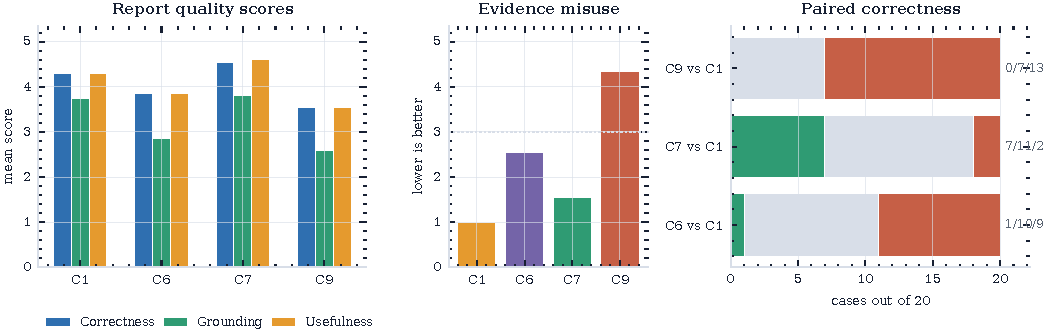
\includegraphics[width=0.98\textwidth]{figures/audit_evidence_human_review_summary.pdf}
    \caption{Pilot human review results. C7 hybrid has the highest average correctness and usefulness, but its grounding advantage over C1 is small and evidence misuse is higher. C6 full white box is worse than C1 on correctness, grounding, and usefulness. C9 shows why correctness alone is insufficient: 11 of 20 shuffled reports have both correctness at least 4 and evidence misuse at least 4. In the paired correctness panel, each label reports better, same, and worse cases relative to C1.}
    \label{fig:human-review}
\end{figure*}

\begin{figure*}[t]
    \centering
    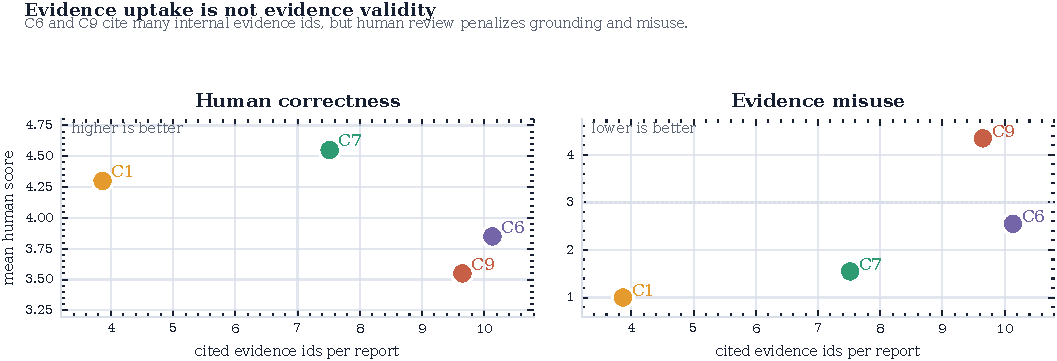
\includegraphics[width=0.98\textwidth]{figures/audit_evidence_uptake_validity.pdf}
    \caption{Evidence uptake is not evidence validity. The x axis uses structural citation volume over the full 60 case run, while the y axes use pilot human review over the 20 paired cases. C6 and C9 cite many evidence ids, but C6 has lower human correctness than C1 and C9 has high evidence misuse. C7 is the strongest condition on correctness, but it still has more misuse than C1.}
    \label{fig:uptake-validity}
\end{figure*}

\section{Qualitative Evidence From Human Review}

The aggregate result is easiest to interpret through actual policy passages. We use the case studies to check whether the numeric pattern means what the paper claims: hybrid evidence can help when passage anchors remain primary, while white box evidence can still mislead when internal labels are treated as substantive policy evidence.

The first case explains why the hybrid interface is useful. Articles 29 and 30 of the Chinese Algorithmic Recommendation Provisions contain two separate issues: confidentiality for supervision bodies and personnel, and a complaint or report mechanism for organizations and individuals. C1 is correct but underemphasizes complaint handling (4, 4, 4, 1). C6 finds a related confidentiality theme but over narrows the report toward legal liability (3, 2, 3, 3). C7 keeps the passage anchored black box surface evidence visible, so the report covers both confidentiality and complaint handling while using internal evidence secondarily (5, 4, 5, 1). C9 is partly correct but cites shuffled transparency evidence (3, 2, 3, 5). This supports the interface claim: hybrid helps because it anchors white box evidence to the passage, not because internal evidence alone supplies the policy interpretation.

The second case shows the limitation. The EU AI Act passage is a classification exception: an Annex III system is not considered high risk if it does not pose a significant risk under listed conditions, but profiling of natural persons remains always high risk. C1 captures the not high risk exception and the profiling carve out (4, 4, 4, 1). C6 turns the classification rule into an obligation like claim (3, 2, 3, 3). C7 improves over C6 but still uses imprecise low risk language (3, 3, 3, 2). C9 uses shuffled deployment evidence and misses the profiling override (2, 2, 2, 5). This is why the paper does not claim that hybrid evidence solves legal precision. It performs best on average, but legal category wording remains fragile.

Across the 11 C9 reports with high correctness and high misuse, we observe three recurring patterns. First, the auditor can read the passage correctly while citing internal evidence from another case. Second, broad SAE or logit lens labels can look relevant to the policy family while failing to support the specific actor, obligation, or exception. Third, shuffled evidence can transfer the report toward plausible transparency, deployment, or risk themes that are not the relevant legal structure. These examples justify the shuffled control as more than a sanity check. A policy audit report can be useful at the surface level and still misuse the internal record. For governance uses, that is precisely the dangerous case: a reviewer who only checks whether the conclusion sounds plausible could miss that the cited internal evidence is irrelevant.

\FloatBarrier

\section{Discussion and Limitations}

The results support a design lesson rather than a simple performance claim. Readable internal evidence can be over trusted. Human review repeatedly identifies broad SAE labels, generic logit lens directions, and non specific steering evidence as failure modes. These artifacts can be directionally related to a policy family while failing to ground the specific actor, obligation, exception, or remedy in the passage. The problem is most visible in C6, where the auditor receives internal evidence without a surface anchor and often turns tool labels into substantive legal or policy claims.

The practical hypothesis is that anchoring matters, but the current design does not isolate anchoring from evidence quantity and variety. C7 receives a larger package than C1 and C6, although it cites less white box evidence than C6 in practice and has much lower repair burden. The result is therefore best read as a design signal: surface passage cues appear to keep the report tied to the policy text, but a volume controlled hybrid condition is needed to separate anchoring from package size. For audit design, this means an evidence package should first preserve the passage and black box observations, then attach internal evidence with explicit caveats and relevance checks. C9 shows why those checks are not optional. If an auditor or reviewer would accept the same style of report under shuffled evidence, the interface is producing transparency theater rather than reliable audit evidence.

The intended governance use is therefore narrow. The paper does not propose an automated legal compliance system. It proposes an evidence interface for human or institutional audit workflows: reviewers need to know which evidence was available, what was cited, and whether irrelevant evidence would have produced similar confidence. For technical AI governance, the contribution is an operationalization of access and verification: internal evidence should be packaged, cited, controlled, and scored before it supports policy audit claims. For mechanistic interpretability, the contribution is an application level evaluation of tool outputs: SAE features, logit lens, steering, and activation explanations are judged by downstream use, including negative controls.

The supported contribution is not that white box evidence generally improves audits. The supported contribution is narrower: evidence access changes report behavior, full white box packages can degrade grounded review, hybrid packages are more promising, and shuffled controls reveal misuse that correctness scores can hide.

The human review is a pilot over 20 cases and four conditions, so it should be read as evidence for interface behavior rather than a final benchmark. There is no inter annotator agreement estimate because the diagnostic review uses one adjudicated reviewer. Single tool conditions C2 through C5 and raw AutoInterp C8 are structurally evaluated but not yet human scored. The target model is small, and the auditor is one local model, so auditor specific trust in labeled internal evidence may affect the results. The activation explanation tool is a surrogate rather than a compatible real Activation Oracle. We do not calibrate SAE label quality, logit lens noise, or steering direction quality, so the experiment cannot fully separate interface risk from tool noise. The evidence packages are not volume controlled; future work should add capped hybrid packages, hybrid plus shuffled white box packages, numeric only internal evidence without readable labels, and conditions where internal evidence is visible but not citable. The report normalization and repair process improves structural validity by fixing JSON and evidence id format issues only, but reviewers score repaired records, so the live burden on an auditor may be higher. Finally, AGORA policy passages support policy audit research but do not by themselves define legal compliance judgments.

\section{Conclusion}

White box evidence packages change how an auditor LLM writes policy audit reports, but full white box access alone does not improve pilot audit quality. It increases internal evidence use while weakening grounding and increasing misuse. Hybrid packages are more promising because they keep passage evidence in control and use internal evidence as a secondary signal. The shuffled control shows why this distinction matters: plausible reports can still misuse invalid internal evidence. The broader lesson is that internal access is valuable for policy auditing only when it is treated as evidence to be validated, not as authority to be trusted.

\section*{Impact Statement}

This work aims to improve transparency and evidence quality in policy relevant AI auditing. The main risk is over interpreting internal evidence as legal or causal proof. The paper therefore reports human review, negative controls, and claim boundaries explicitly.

\FloatBarrier

\bibliography{policy_feature_map_refs}
\bibliographystyle{icml2026}

\appendix

\onecolumn

\section{Full Evidence Condition Details}

The experiment compares evidence interfaces, not retrieval systems. Each condition provides the same policy passage and audit rubric, but changes the auditor facing evidence items. \Cref{tab:appendix-condition-details} expands the condition table used in the main paper.

\begin{table}[h]
    \centering
    \caption{Appendix condition details. Citation rules are part of the interface design: passage spans and evidence ids are separate objects.}
    \label{tab:appendix-condition-details}
    \scriptsize
    \begin{tabular}{@{}p{0.08\textwidth}p{0.28\textwidth}p{0.23\textwidth}p{0.27\textwidth}@{}}
        \toprule
        Condition & Auditor input fields & Allowed evidence citation & Expected misuse risk \\
        \midrule
        C0 passage only & Policy passage, visible metadata, and fixed rubric. & Passage spans only. & Unsupported claims may look plausible because no external evidence ids are available. \\
        C1 black box surface & Passage plus surface observations, issue notes, selected spans, and confidence fields. & Black box surface ids and passage spans. & Surface notes may encourage generic legal readings, but evidence remains tied to text. \\
        C2 SAE only & Sparse feature ids, layers, activations, activated spans, labels, review fields, and caveats. & SAE ids and passage spans. & Readable feature labels may be treated as policy conclusions. \\
        C3 logit lens only & Intermediate token direction records at selected layers and positions. & Logit lens ids and passage spans. & Token direction evidence may be overread as a causal explanation. \\
        C4 steering only & Hidden state direction probes with alpha, token changes, and caveats. & Steering ids and passage spans. & Sensitivity evidence may be mistaken for a deployable control or legal proof. \\
        C5 activation explanation surrogate & Natural language activation hypotheses derived from local evidence. & Surrogate explanation ids and passage spans. & Natural language hypotheses can sound authoritative despite being unvalidated. \\
        C6 full white box & SAE, logit lens, steering, and activation explanation surrogate items. & All white box ids and passage spans. & Dense internal evidence can distract from the passage and increase over citation. \\
        C7 hybrid & C1 surface evidence plus C6 white box evidence. & Black box ids, white box ids, and passage spans. & Best practical interface in the pilot, but still vulnerable to internal evidence overuse. \\
        C8 raw AutoInterp SAE & Raw SAE labels and feature ids without the surrounding package context. & Raw SAE ids and passage spans. & Label readability may hide missing context and caveats. \\
        C9 shuffled white box control & C6 style white box evidence from another case, hidden from the auditor. & Shuffled white box ids and passage spans. & Measures whether plausible internal evidence is trusted when relevance is broken. \\
        \bottomrule
    \end{tabular}
\end{table}

\section{Tool Construction Details}

This appendix defines the evidence artifacts exposed to the auditor. These details matter because the experiment evaluates interfaces, not the intrinsic correctness of any one interpretability tool.

\paragraph{Black box surface evidence.} C1 contains no hidden state information. The passage is split into sentences, and each sentence is scored by the audit cue count $b(s)$ in the main text. The cue lexicon includes obligation, prohibition, risk, safety, security, transparency, monitoring, assessment, testing, threshold, compliance, enforcement, provider, operator, user, deploy, market, harm, vulnerable, and fundamental rights terms. The five highest scoring sentences become evidence items with ids such as \texttt{BB\_SURFACE\_1}. Each item stores the sentence index, matched cue count, a supporting passage span, and the caveat that the item is extractive surface evidence.

\paragraph{SAE evidence.} For Gemma 2 2B residual states, Gemma Scope SAE features are summarized as candidate concept activations. For feature $k$ at layer $l$, the package records
\begin{equation}
A_{i,l,k}=\max_{p} a_{i,l,k,p}, \qquad p^{*}_{i,l,k}=\arg\max_{p} a_{i,l,k,p}.
\end{equation}
Features with nonzero activation are sorted by activation score, capped to a compact set, and rendered with layer, feature id, peak token, activated span, model id, SAE release, and caveat. In C2, C6, and C7, labels use human revised AutoInterp where the review marked the label usable or preserved. C8 exposes raw AutoInterp style labels without that review layer.

\paragraph{Logit lens evidence.} Logit lens positions are selected from audit cue token offsets in the passage, with a fallback to the final active token. At layers $l\in\{6,12,18,24\}$, the package computes $\ell_{i,l,p}=W_U\mathrm{LN}(h_{i,l,p})$ and records the top five vocabulary tokens and scores. These items are evidence about intermediate token directions, not evidence that the model finally predicts or endorses those tokens.

\paragraph{Steering evidence.} Steering directions are constructed from positive prompts about obligations, risk controls, compliance duties, monitoring, transparency, accountability, enforcement, and harm protection, contrasted with negative prompts describing background text without binding duties. For each layer $l\in\{12,18,24\}$,
\begin{equation}
v_l=\frac{\mu_l^{+}-\mu_l^{-}}{\|\mu_l^{+}-\mu_l^{-}\|_2}, \qquad
h'_{i,l,p}=h_{i,l,p}+0.35\|h_{i,l,p}\|_2v_l.
\end{equation}
The package records base and steered top tokens, whether the top token changes, and the KL divergence between base and steered vocab distributions. It does not run a full generation under intervention.

\paragraph{Activation explanation surrogate.} The activation explanation condition is a conservative surrogate. It converts selected SAE labels, activations, peak tokens, and spans into a short activation meaning hypothesis with low confidence metadata. The item is explicitly labeled as a surrogate so that the auditor cannot treat it as a validated Activation Oracle output.

\paragraph{Shuffled control.} C9 keeps the target policy passage fixed but shifts full white box packages across cases. Thus $x_i$ is paired with $\package_{j,\mathrm{C6}}$ for $j\neq i$ while the auditor sees only a normal full white box shaped package. The control tests whether relevance is being checked or whether plausible internal evidence is being cited because it looks audit like.

\section{Audit Prompt and Report Schema}

The auditor prompt is designed to make traceability a first class output rather than a later reconstruction. The prompt states that the policy passage is the primary source of truth and that evidence items are hypotheses or pointers. The auditor must return raw JSON, cite exact short passage spans, avoid invented evidence ids, and avoid causal claims from one tool alone.

\begin{verbatim}
{
  "summary": "one concise paragraph",
  "issue_findings": [
    {
      "issue_tag": "short audit issue label",
      "finding": "what the auditor should notice",
      "actor": "responsible actor if present",
      "obligation_or_risk": "obligation, risk, or gap",
      "supporting_policy_spans": ["exact short spans from the passage"],
      "evidence_ids": ["evidence ids used, if any"],
      "confidence": 0.0,
      "uncertainty": "main limitation or missing information"
    }
  ],
  "confounds_or_alternatives": ["plausible alternative readings"],
  "internal_evidence_used": ["evidence ids that materially changed the audit"],
  "unsupported_or_low_confidence_claims": [
    "claims that should not be over stated"
  ],
  "overall_confidence": 0.0
}
\end{verbatim}

The schema separates three evidence objects: the policy passage, condition specific evidence ids, and the auditor's own claims. This separation is what makes shuffled evidence failures visible. A report can have correct passage claims while still citing invalid internal evidence.

\section{Human Gold Review Protocol}

Human review has two stages. First, gold briefs are written from the policy passage and source metadata without seeing model reports or evidence packages. Each gold brief records issue tags, actors, obligations, support spans, known confounds, and unsupported claims to penalize. Second, diagnostic review scores auditor reports against the gold brief for four conditions: C1, C6, C7, and C9.

For each reviewed report, the diagnostic vector is
\begin{equation}
h_{i,c}=(h^{\mathrm{corr}}_{i,c},h^{\mathrm{ground}}_{i,c},h^{\mathrm{use}}_{i,c},h^{\mathrm{misuse}}_{i,c}).
\end{equation}
The first three coordinates reward match to the gold brief, while the fourth penalizes invalid evidence use. This means a report can be high quality on passage interpretation and still fail as an audit evidence artifact if $h^{\mathrm{misuse}}_{i,c}$ is high. The C9 analysis focuses on exactly this conjunction.

\begin{table}[h]
    \centering
    \caption{Human review axes and claim boundaries.}
    \label{tab:appendix-human-review-protocol}
    \small
    \begin{tabular}{p{0.19\textwidth}p{0.39\textwidth}p{0.34\textwidth}}
        \toprule
        Axis & Measures & Does not measure \\
        \midrule
        Correctness & Match to the gold issue, actor, and obligation structure. & Whether the target model actually used the cited internal feature causally. \\
        Span grounding & Whether major claims are tied to concrete passage spans. & Whether the cited span is sufficient for a legal decision outside the passage. \\
        Diagnostic usefulness & Whether the report would help an auditor notice the policy issue or gap. & Whether the report is a complete compliance analysis. \\
        Evidence misuse & Whether the report overreads, overcites, or relies on irrelevant internal evidence. & Whether the passage level claim is necessarily wrong. \\
        \bottomrule
    \end{tabular}
\end{table}

\section{All Condition Structural Summary}

\begin{figure}[h]
    \centering
    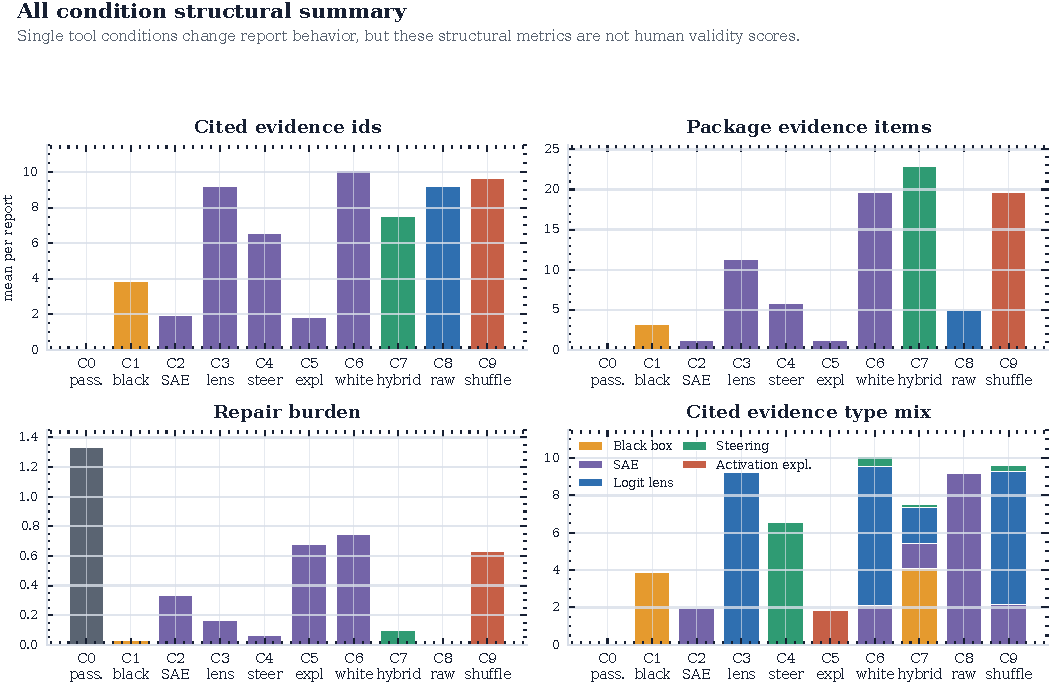
\includegraphics[width=0.94\textwidth]{figures/audit_evidence_condition_summary.pdf}
    \caption{Structural metrics across all ten evidence conditions. Single tool conditions change citation behavior and repair burden, but these measures are not human validity scores. C3 and C8 show high citation volume under single tool interfaces, while C9 shows that a full white box shaped package can be cited heavily even when relevance is broken.}
    \label{fig:appendix-structural-summary}
\end{figure}

\section{Case Study 1: Hybrid Anchoring Works}

This case uses Articles 29 and 30 of the Internet Information Service Algorithmic Recommendation Management Provisions. The passage contains two distinct policy issues: confidentiality duties for bodies and personnel involved in supervision, and a complaint or report mechanism for organizations and individuals.

\begin{quote}
\small
Article 29: Related bodies and personnel participating in algorithmic recommendation service security assessment, supervision, and inspection shall maintain confidentiality of the personal private information, personal information, and commercial secrets they learn when exercising their duties and responsibilities, they may not disclose, sell, or illegally provide it to other persons. Article 30: Where any organization or individual discovers acts violating these Provisions, they may file a complaint or report with cybersecurity and informatization departments and relevant departments. Departments receiving complaints or reports shall handle them timely and according to the law.
\end{quote}

The gold brief identifies confidentiality in supervision, complaint and report rights, and complaint handling obligations. \Cref{tab:appendix-cn21-case} shows why C7 is a better interface for this case. The important point is not that white box evidence alone solves the interpretation. C6 narrows the report to confidentiality and legal liability, while C7 keeps the surface anchors that identify both Article 29 and Article 30.

\begin{table}[h]
    \centering
    \caption{Case study 1 diagnostic comparison for \texttt{chinese\_algorithmic\_recommendation\_rules\_266\_21}. Scores are correctness, grounding, usefulness, and misuse. Lower misuse is better.}
    \label{tab:appendix-cn21-case}
    \scriptsize
    \begin{tabular}{p{0.08\textwidth}p{0.30\textwidth}p{0.24\textwidth}p{0.24\textwidth}}
        \toprule
        Condition & Report behavior & Cited evidence pattern & Human interpretation \\
        \midrule
        C1 & Identifies confidentiality and mentions accountability, but the first finding centers on confidentiality. & Uses \texttt{BB\_SURFACE\_1}, \texttt{BB\_SURFACE\_2}, and \texttt{BB\_SURFACE\_3}. & 4, 4, 4, 1. Correct but mildly emphasizes unspecified enforcement gaps. \\
        C6 & Captures confidentiality but omits the complaint and report mechanism. The summary leans toward legal liability. & Uses logit lens ids at the obligation token position. & 3, 2, 3, 3. Logit only evidence is weak and the report overstates the liability theme. \\
        C7 & Covers confidentiality, nondisclosure, complaint or report rights, and handling by departments. & Uses the three black box surface anchors, while white box evidence remains secondary. & 5, 4, 5, 1. Best result because the passage anchors preserve both Articles 29 and 30. \\
        C9 & Produces a partially correct confidentiality finding but cites shuffled transparency evidence. & Uses \texttt{SAE\_L12\_F12255} and shuffled logit and steering ids. & 3, 2, 3, 5. The internal evidence is mismatched even though the passage claim is partly correct. \\
        \bottomrule
    \end{tabular}
\end{table}

\section{Case Study 2: White Box Can Misframe Legal Category}

This case uses an EU AI Act provision on high risk classification exceptions. The passage is legally delicate because it is not a generic operator duty. It specifies when an Annex III system is not considered high risk, while preserving an override for profiling of natural persons.

\begin{quote}
\small
By derogation from paragraph 2, an AI system referred to in Annex III shall not be considered to be high risk where it does not pose a significant risk of harm to the health, safety or fundamental rights of natural persons, including by not materially influencing the outcome of decision making. The first subparagraph shall apply where any listed condition is fulfilled, including a narrow procedural task, improving a previously completed human activity, detecting decision making patterns without replacing or influencing the prior human assessment without proper human review, or performing a preparatory task. Notwithstanding the first subparagraph, an AI system referred to in Annex III shall always be considered to be high risk where the AI system performs profiling of natural persons.
\end{quote}

The gold brief identifies a classification exception, a significant risk threshold, decision making influence, Annex III scope, and a profiling override. \Cref{tab:appendix-eu21-case} shows a limitation of the hybrid result: even C7 can shift to imprecise legal wording. This case keeps the paper's claim boundary intact. Hybrid is promising on average, not a guarantee of legal category precision.

\begin{table}[h]
    \centering
    \caption{Case study 2 diagnostic comparison for \texttt{eu\_high\_risk\_ai\_governance\_757\_21}. Scores are correctness, grounding, usefulness, and misuse. Lower misuse is better.}
    \label{tab:appendix-eu21-case}
    \scriptsize
    \begin{tabular}{p{0.08\textwidth}p{0.30\textwidth}p{0.24\textwidth}p{0.24\textwidth}}
        \toprule
        Condition & Report behavior & Cited evidence pattern & Human interpretation \\
        \midrule
        C1 & Captures non high risk exceptions and the profiling carve out. & Uses surface evidence ids tied to passage spans. & 4, 4, 4, 1. Correct but could state more clearly that this is classification criteria. \\
        C6 & Recasts the rule as an obligation to consider systems non high risk. & Uses logit lens ids around selected token positions. & 3, 2, 3, 3. Partially correct but turns a legal classification rule into an obligation. \\
        C7 & Captures conditions and profiling but uses low risk wording. & Mainly uses black box surface ids despite receiving white box evidence. & 3, 3, 3, 2. Hybrid helps but the legal category is less precise than not high risk. \\
        C9 & Infers a risk assessment gap and misses the mandatory profiling carve out. & Uses shuffled deployment evidence and unrelated logit ids. & 2, 2, 2, 5. Control evidence is mismatched and the key exception structure is lost. \\
        \bottomrule
    \end{tabular}
\end{table}

\section{Shuffled Control Failure Table}

\Cref{tab:appendix-c9-failures} lists the 11 C9 reports with correctness at least 4 and evidence misuse at least 4. These are the most important governance failures because a reviewer who checks only passage level correctness could miss the invalid internal evidence use.

\begin{table}[h]
    \centering
    \caption{C9 cases with plausible correctness and high evidence misuse.}
    \label{tab:appendix-c9-failures}
    \scriptsize
    \begin{tabular}{@{}p{0.07\textwidth}p{0.14\textwidth}p{0.24\textwidth}p{0.15\textwidth}p{0.25\textwidth}@{}}
        \toprule
        Case & Source & Gold issue & Shuffled evidence cited & Reviewer finding \\
        \midrule
        CN 12 & Chinese AR Provisions & User notice, transparency, service mechanism disclosure. & Logit lens. & Substantively close, but control evidence is not reliable support. \\
        CN 13 & Chinese AR Provisions & Non targeted option, switch off right, tag controls, explanation for major rights impacts. & SAE and logit lens. & Mostly right, but depends on control evidence and compresses distinct remedies. \\
        CN 14 & Chinese AR Provisions & Minor protection, beneficial content, harmful content restriction, addiction prevention. & SAE and logit lens. & Correct surface conclusion despite mismatched control evidence. \\
        CN 24 & Chinese AR Provisions & Filing fraud sanctions, filing cancellation, administrative penalties. & SAE and logit lens. & Close to the passage, but control evidence should not be treated as support. \\
        CN 7 & Chinese AR Provisions & Information security, unlawful content handling, records preservation. & SAE. & Good surface summary, but control SAE labels are generic and mismatched. \\
        EU 182 & EU AI Act & Right to explanation and high risk AI deployer obligation. & SAE and logit lens. & Primary obligation is correct, but control evidence is mismatched and exceptions are missing. \\
        EU 200 & EU AI Act & Administrative fines and SME fine cap. & Logit lens. & Substantively correct but control evidence is not trustworthy support. \\
        EU 231 & EU AI Act & Technical documentation, validation, logs, cybersecurity measures. & Logit lens. & Mostly correct, but evidence is invalid and the report is thinner on testing logs. \\
        EU 28 & EU AI Act & Risk management system across lifecycle and foreseeable misuse. & Logit lens. & Correct on continuous risk management, but shuffled evidence should not be accepted. \\
        EU 38 & EU AI Act & Human oversight and risk minimization. & SAE. & Substantively accurate, showing generic shuffled labels can look persuasive. \\
        EU 83 & EU AI Act & Notified body designation restriction and certificate actions. & SAE and logit lens. & Correct assessment claim, but evidence is plainly mismatched and incomplete. \\
        \bottomrule
    \end{tabular}
\end{table}

\section{Pilot Human Review Case Matrix}

\Cref{tab:appendix-case-matrix} reports the case level correctness and misuse scores used in the main result. Each cell is correctness/misuse. Higher correctness is better, lower misuse is better. The table shows why the mean result should be read as an interface pattern rather than a universal quality claim: C7 is often strongest, but some legal category cases remain difficult and C9 can be plausibly correct while misusing evidence.

\begin{table}[h]
    \centering
    \caption{Pilot case matrix. Each cell is correctness/evidence misuse.}
    \label{tab:appendix-case-matrix}
    \scriptsize
    \begin{tabular}{p{0.10\textwidth}p{0.35\textwidth}rrrr}
        \toprule
        Case & Source & C1 & C6 & C7 & C9 \\
        \midrule
        CN 12 & Chinese AR Provisions & 4/1 & 5/2 & 5/2 & 4/4 \\
        CN 13 & Chinese AR Provisions & 5/1 & 4/2 & 5/1 & 4/4 \\
        CN 14 & Chinese AR Provisions & 4/1 & 4/3 & 5/2 & 4/4 \\
        CN 15 & Chinese AR Provisions & 4/1 & 4/3 & 4/2 & 3/4 \\
        CN 21 & Chinese AR Provisions & 4/1 & 3/3 & 5/1 & 3/5 \\
        CN 24 & Chinese AR Provisions & 4/1 & 4/3 & 4/2 & 4/4 \\
        CN 5 & Chinese AR Provisions & 5/1 & 4/3 & 5/2 & 3/5 \\
        CN 6 & Chinese AR Provisions & 4/1 & 4/2 & 5/1 & 3/4 \\
        CN 7 & Chinese AR Provisions & 5/1 & 3/3 & 5/1 & 4/4 \\
        CN 9 & Chinese AR Provisions & 3/1 & 3/4 & 3/3 & 2/5 \\
        EU 182 & EU AI Act & 4/1 & 4/2 & 5/1 & 4/4 \\
        EU 2 & EU AI Act & 4/1 & 3/3 & 4/2 & 3/5 \\
        EU 200 & EU AI Act & 5/1 & 4/2 & 5/1 & 4/4 \\
        EU 21 & EU AI Act & 4/1 & 3/3 & 3/2 & 2/5 \\
        EU 231 & EU AI Act & 4/1 & 3/3 & 5/2 & 4/4 \\
        EU 28 & EU AI Act & 5/1 & 5/2 & 5/1 & 5/4 \\
        EU 30 & EU AI Act & 4/1 & 4/2 & 5/1 & 3/5 \\
        EU 38 & EU AI Act & 5/1 & 5/2 & 4/1 & 5/4 \\
        EU 39 & EU AI Act & 4/1 & 4/2 & 4/2 & 3/4 \\
        EU 83 & EU AI Act & 5/1 & 4/2 & 5/1 & 4/5 \\
        \bottomrule
    \end{tabular}
\end{table}

\section{Human Review Score Distributions}

\Cref{tab:appendix-score-distributions} reports the score distributions behind the means. Each vector lists counts for scores 1 through 5. The distributions make the same claim boundary visible: C7 has more high correctness and usefulness scores than C1, but it also shifts misuse upward; C9 remains often plausible on correctness while all shuffled reports score 4 or 5 on misuse.

\begin{table}[h]
    \centering
    \caption{Pilot human review score distributions. Each vector is counts for scores 1/2/3/4/5.}
    \label{tab:appendix-score-distributions}
    \scriptsize
    \setlength{\tabcolsep}{3pt}
    \begin{tabular}{@{}lrrrr@{}}
        \toprule
        Condition & Correct & Ground & Useful & Misuse \\
        \midrule
        C1 & 0/0/1/12/7 & 0/0/5/15/0 & 0/0/1/12/7 & 20/0/0/0/0 \\
        C6 & 0/0/6/11/3 & 0/6/11/3/0 & 0/0/6/11/3 & 0/10/9/1/0 \\
        C7 & 0/0/2/5/13 & 0/0/4/16/0 & 0/0/2/4/14 & 10/9/1/0/0 \\
        C9 & 0/2/7/9/2 & 0/8/12/0/0 & 0/2/7/9/2 & 0/0/0/13/7 \\
        \bottomrule
    \end{tabular}
\end{table}

\section{Reproducibility Notes}

The anonymized artifact repository for this paper is available at \url{https://anonymous.4open.science/r/agora-mi-C473/README.md}.

The active report file contains 600 JSONL records, one for each condition case pair. Structural summaries are computed from the final quality check CSV. Human review summaries are computed from the diagnostic review sheet and the human review summary JSON file. The main paper reports only values that appear in those summary artifacts. The appendix case studies use the human gold brief, diagnostic review sheet, and final structured report records for the named case ids.

Citation validity is a structural check:
\begin{equation}
V_{i,c}=\mathbf{1}\left[ Z_{i,c}\subseteq \{id(e):e\in\package_{i,c}\}\right].
\end{equation}
The reported value 1.0 means cited ids are valid members of the supplied package after the repair pass. It does not mean that the cited evidence is substantively relevant, which is why C9 can have perfect citation validity and high human scored misuse. Report repair is restricted to JSON parsing, schema normalization, confidence normalization, and evidence id cleanup; it does not change the policy passage, evidence package, or substantive report findings.

All reported numeric claims should be regenerated from three artifact classes: the final report JSONL, the structural summary CSV, and the human review summary files. The manuscript intentionally avoids model self grading and retrieval proxy metrics. The only quality numbers in the main text come from human diagnostic review.

\end{document}
